%!TEX root = ../main.tex

\chapter{Background}
\label{chp:background}

\section{Methodological Background}
\subsection{Resource Description Framework}
The \ac{RDF} is a standard\footnote{https://www.w3.org/RDF/} by the World Wide Web Consortium (W3C) designed for data interchange on the web. Its definitive syntax was lastly defined on 2003 \cite{beckett2004rdf}.

\ac{RDF} is based on the idea of making statements about resources, expressed as triples: for example, a triple might consist of "Gene123" (subject) "hasFunction" (predicate) "DNA Repair" (object). These triples are stored in a graph, making \ac{RDF} uniquely suited for modern data analytics where relationships and linkages are crucial: this structure is by design flexible, and it is used to represent information in a way that makes it easier to aggregate, integrate, and manage diverse data from various sources.

The standard utilizes \ac{URI} to ensure that each element in the triple is uniquely identifiable, allowing to link data across different datasets seamlessly. \ac{RDF} also supports literal values and datatypes, enabling detailed descriptions of properties and values.

In summary, \ac{RDF} provides a robust and flexible framework for describing and interlinking data on the web, which is crucial for any federated data system that aims to integrate diverse data sources effectively.

\subsection{Knowledge Graphs}
Knowledge Graphs represent an innovative way of structuring and querying interconnected data. A \ac{KG} organizes data in a graph format, where entities (nodes) and their interrelations (edges) are defined according to a schema that encapsulates both the entities and the possible links between them. This structure allows not only to better visualize data, but is also very well suited for data exploration and analysis.

Central to the concept of \ac{KG} is the idea of enhancing search and data discovery capabilities beyond simple data retrieval. By semantically linking data entities, \ac{KG} allow for more intuitive and sophisticated queries that are closer to natural language questions. This capability makes them useful in complex domains like biomedical research, where users may need to uncover hidden relationships and patterns among vast datasets.

Furthermore, \ac{KG} well suits in scenarios requiring data integration from disparate sources. They support the combination of structured and unstructured data and they can scale well as new data need to be integrated. This flexibility is crucial in fields such as genomics, where new data attributes and relationships are continuously being discovered and need to be rapidly integrated into existing datasets.

In practice, \ac{KG} are usually powered by technologies such as \ac{RDF} and other standards discussed earlier, leveraging the strengths of these frameworks to ensure robust data handling and scalability.

\subsection{Ontologies}
Ontologies are a shared vocabulary for a particular domain. They serve as a crucial tool in structuring data by defining classes where data entities can be categorized. This classification system not only standardizes data representation but also simplifies the communication between different systems and users by providing a common understanding of the domain.

Ontologies involve the use of first-order logic to define rules about the relationships between different classes. These rules allow for the logical inference of new information from the data that is already known, which can significantly deepen data analysis and querying capabilities. This set of first-order logic rules used to model ontologies composes the \ac{OWL} \cite{mcguinness2004owl}.

With ontologies integrated within a \ac{KG}, it is possible to employ inferential algorithms either at query time or at preprocessing time. This capability enables the derivation of new knowledge that isn't explicitly stated in the data but can be inferred based on the ontological representations.

The use of ontologies in a \ac{KG} is crucial in complex domains like genomics. Here, the ability to infer new relationships and properties can lead to understanding intricate biological connections and processes.

In summary, ontologies provide the foundational structure for managing complex information systems. They not only facilitate a standardized approach to data handling and integration but also enhance the capability of systems to derive and utilize new knowledge effectively.

\subsection{Data Federation} \label{DF}
Data Federation is a technology that organizes data from multiple different and autonomous data sources and makes it accessible under a uniform data model, allowing for real-time data retrieval from various sources without requiring data deduplication. This approach creates a unified data access layer that abstracts the underlying technical details of each \ac{DBMS}. Users can query this virtual layer using standard data querying languages, like \ac{SQL}, without needing to know where the data is physically stored or in what format.

A key strength of Data Federation lies in its capacity to harmonize heterogeneous data sources, ranging from traditional relational databases to modern big data solutions and cloud services. This integration is seamless and dynamic, scaling well as soon as new sources come in, without requiring significant reconfiguration. Such agility is crucial in fields like genomics, where data formats and sources evolve rapidly alongside scientific advancements. Moreover, it minimizes the risks associated with data duplication and movement, such as data loss or corruption. It also ensures that data remains current, reflecting real-time changes without delay. This is particularly valuable for decision-making processes where up-to-date information is critical.

Different existing Data Federation systems may have different characteristics, and the choice of which system suits better certain requirements may depend on many different factors. A recent comparative study on Data Virtualization Systems \cite{DBLP:journals/semweb/GuCLMXXC24} highlights and evaluates diverse features of many systems coming both from the academia as well enterprise solutions, such as supported query languages, supported data sources, data security, exposed interfaces and software support.

\subsection{Semantic Data Integration}
Semantic Data Integration is an approach that aims to integrate data from a single relational source to an ontology that models a specific domain. This integration is achieved by defining mappings that establish semantic relationships among data entities.

The core idea behind semantic data integration involves establishing a global schema, represented by the ontology, which acts as a blueprint for how data from various sources is viewed and accessed. This ontology defines not just the entities and their attributes but also the relationships and constraints between these entities. The mapping between the ontology (global schema) and the relational data source is critical as it dictates how data is interpreted in a meaningful way.

The concept of Data Integration, firstly introduced without a semantic focus \cite{DBLP:conf/pods/Lenzerini02}, has evolved with research advancements in this field. These advancements have led to the development of tools and mapping languages specifically designed for semantic data integration, laying the groundwork for a paradigm known as \ac{OBDA} \cite{DBLP:conf/ijcai/XiaoCKLPRZ18}.

The \ac{OBDA} framework, that has been precisely formalized \cite{DBLP:conf/aiia/BotoevaCCCX18}, is composed of a chain of procedures that can be summarized as follows:
\begin{enumerate}
    \item input query ${q(\vec{x})}$ is rewritten \cite{DBLP:conf/otm/MakrisGBC10} into ${q'}$ over the virtual ABox ${A'}$ (i.e. the first-order logic specification of the ontology);
    \item the rewritten query ${q'}$ is unfolded using the \textit{mappings} into an \ac{SQL} query ${q^*}$;
    \item the optimised SQL query ${q^*}$ is evaluated over the data instance ${D}$ (e.g. a relational \ac{DBMS}).
\end{enumerate}

Figure \ref{fig:OBDAframew} outlines the aforementioned algorithm within a flowchart.

\begin{figure}[ht]
    \centering
    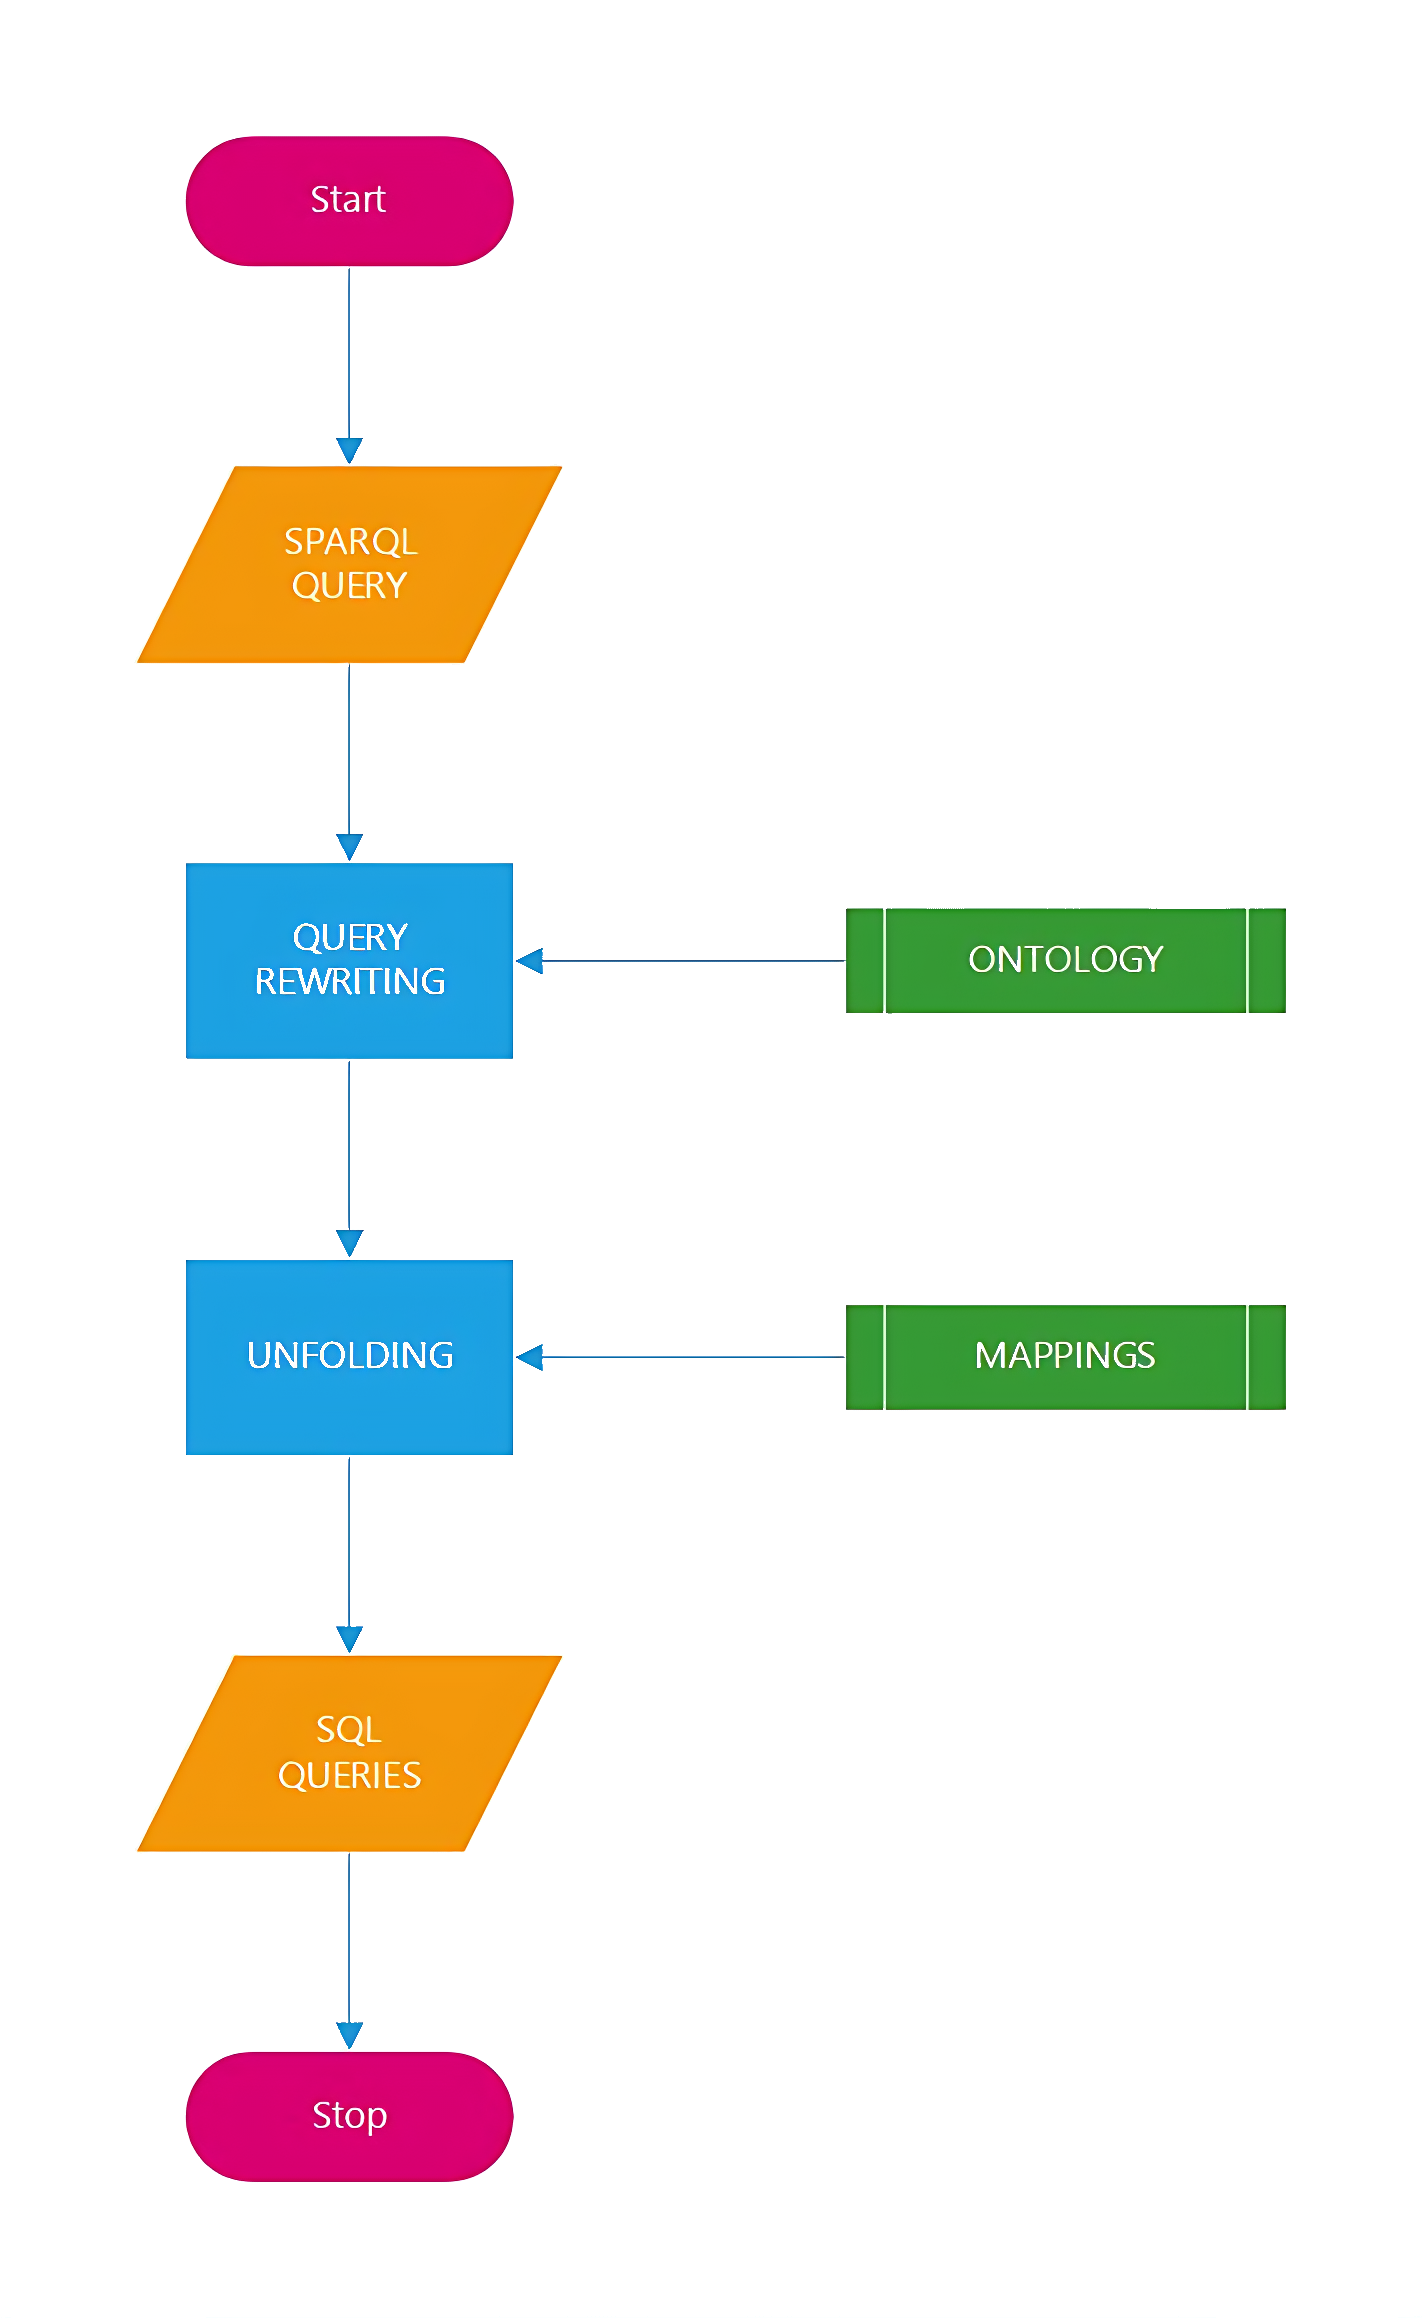
\includegraphics[width=8cm]{res/obda_framework.png}
    \caption{The OBDA framework}
    \label{fig:OBDAframew}
\end{figure}


\section{Technical Background}
\subsection{Data Federation Systems}
As discussed in section \hyperref[DF]{2.1.4}, Data Federation Systems are sophisticated softwares and thus evaluable under many aspects. In this background analysis we will focus on four main aspects, considering their importance as the Data Federation System will be part of a broader framework. In particular, by the aforementioned comparison, we will present three most prominent systems considering:
\begin{itemize}
    \item software support \& documentation;
    \item scalability;
    \item logging capabilities;
    \item performances.
\end{itemize}

These features are also briefly summarized in Tab. \ref{tab:comparison}.

\subsubsection{Denodo}
Denodo\footnote{https://denodo.com/en} is an enterprise virtualization platform that serves as a data federation system, integrating data from diverse sources to provide a unified view without requiring physical data deduplication. It allows for real-time access to structured and unstructured data from various sources including relational, column and No-SQL databases, web \ac(API), and flat files.

Denodo provides robust security features, including hashing, encrypting functions and user privileges, ensuring that sensitive data is protected according to compliance standards.

Moreover, it utilizes advanced query optimization techniques, such as caching and query rewriting, to enhance performance. These optimizations ensure efficient data retrieval, reducing latency and improving the overall speed of data access across the federated sources.

Although it is highly scalable, capable of accommodating new data sources, and it is provided also with a custom source wrapper template for unsupported data sources, being it an enterprise solution allows for maximum five connections, unless a premium plan is signed.

\subsubsection{Teiid}
Teiid\footnote{https://teiid.io/} is an open-source Java component developed by Red Hat\footnote{https://www.redhat.com/} that provides integrated access to multiple data sources through a single uniform API. Rather than a \ac{DBMS}, Teiid is more a query engine for integrating data from multiple sources, accessible both through \ac{API} and \ac{JDBC}/\ac{ODBC} interfaces.

It comes in different shapes: there are Teiid implementations as an Eclipse plugin as well as deployable packages on web containers such as Wildfly and OpenShift.

One of the main issues with Teiid is poor documentation when it is not deployed alongside enterprise solutions (like OpenShift). Moreover, no major releases have been published since four years, and many open issues on the official GitHub repository\footnote{https://github.com/teiid/teiid} are not being addressed.

\subsubsection{Dremio}
Similarly to Denodo, Dremio\footnote{https://www.dremio.com/} is a virtualization platform that serves as a data federation system. Although it is developed within an enterprise context, the standard version, comprehensive of most of the Dremio features, it is \ac{FOSS} under the Apache 2.0 license, combining typical enterprise software robustness with a strong community active on continuous maintenance.

Even if it is possible to use Dremio as a standalone instance (e.g. on a server), it is by design a distributed system and thus it can run on clusters up to more than 1000 nodes. In case of standalone configurations, in linux server environments it is possible to install it using packet managers, but the easiest way is to use the Docker image it comes with.

Dremio makes use of Apache Arrow to enhance processing speeds and reduce latency. Moreover, it optimizes query performance through its advanced query planner and execution engine, which can push down operations to the data source level, minimizing data movement and speeding up response times.

It provides comprehensive security features that include encryption, access controls, and data masking to ensure privacy. It also maintains detailed logs of all queries, which are crucial for compliance purposes in many fields such as the clinical domain, where patient medical data is managed alongside their personal information.

As in Denodo, but under an open-source perspective, it is possible to build custom connectors for unsupported data sources and Dremio. This is realizable through \ac{ARP} connectors: a public repository\footnote{https://github.com/dremio-hub/dremio-sqllite-connector} provides a Maven template, that is customizable for each data source for which a \ac{JDBC} driver is available.

In conclusion, Dremio offers an open-source virtualization system with the typical robustness of enterprise softwares; it is highly scalable both in the sense of computation distribution over clusters and in the types of supported sources, and it has a comprehensive logging system that suits well for tracking data flow.

\begin{table}[ht]
    \centering
    \begin{tabular}{| p{0.2\linewidth} | p{0.12\linewidth} | p{0.12\linewidth} | p{0.12\linewidth} | p{0.15\linewidth} | p{0.12\linewidth} |}
    \hline
    \textbf{} & \textbf{Support} & \textbf{Free and Open Source} & \textbf{Well Documented} & \textbf{Scalability} & \textbf{Solid Logging Capabilities}\\ \hline
    \raisebox{-0.3\height}{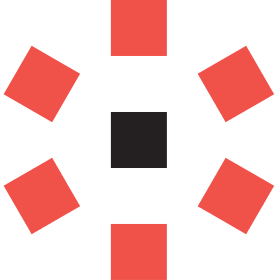
\includegraphics[width=0.6cm]{res/denodo.png}} Denodo  & ✓ &  & ✓ & ✓ & ✓ \\ \hline
    \raisebox{-0\height}{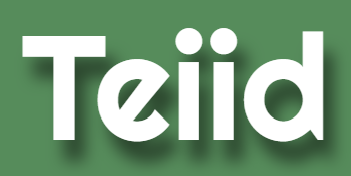
\includegraphics[width=0.6cm]{res/teiid.png}} Teiid   &  & ✓ &  &  &  \\ \hline
    \raisebox{-0.3\height}{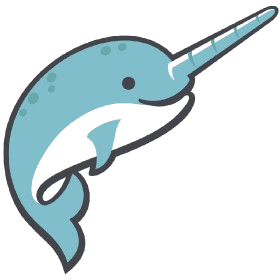
\includegraphics[width=0.6cm]{res/dremio.png}} Dremio  & ✓ & ✓ & ✓ & ✓ & ✓\\ \hline
    \end{tabular}
    \caption{Comparative among Data Federation Systems \label{tab:comparison}}
\end{table}


\subsection{OBDA Systems}
\ac{OBDA}, as shown in Fig. \ref{fig:obda_two}, allows to seamlessly integrate a relational source within an ontology, so to add a semantic layer. Research on this specific topic has been performed not only by the academy, but also from Research \& Development branches of big companies, considering the impact on the industry: a preliminary analysis \cite{DBLP:conf/semweb/KharlamovSOZHLRSW14} by Siemens\footnote{https://www.siemens.com/} that lead subsequently to a custom platform, analyzed existing systems. Table \ref{tab:obda_comparison} summarizes the content of this analysis.

\begin{figure}[ht]
    \centering
    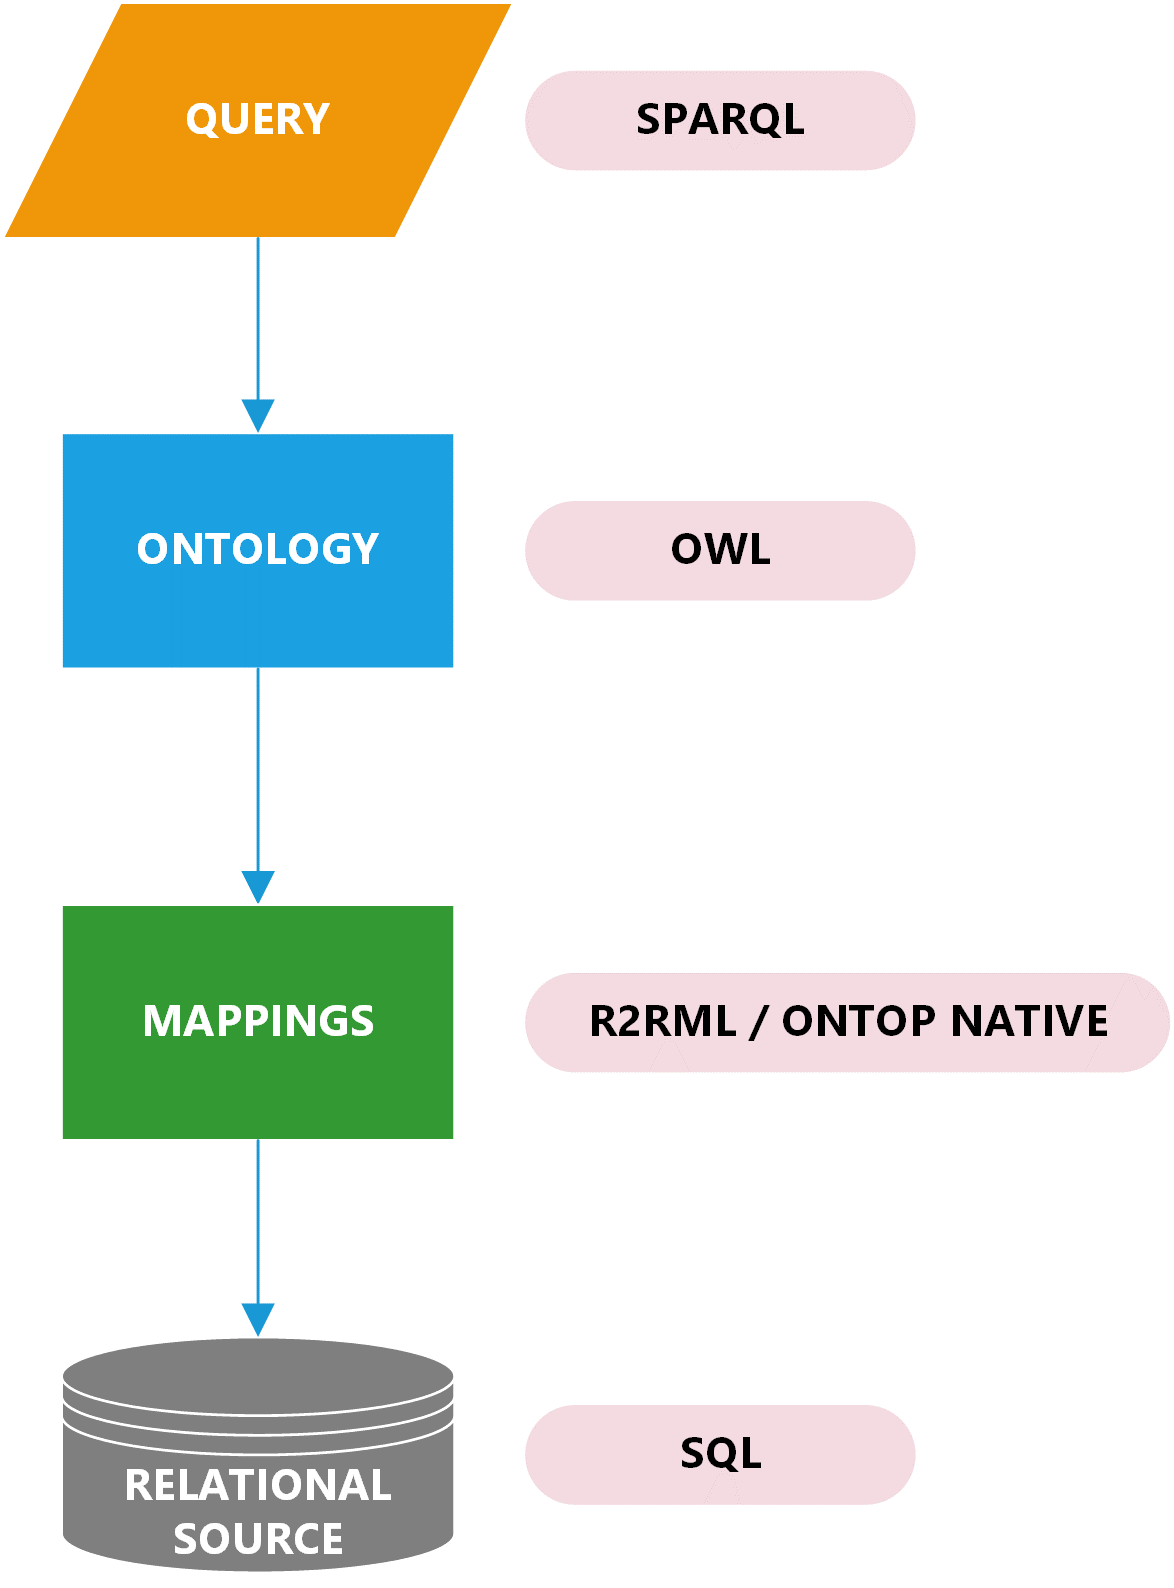
\includegraphics[width=8cm]{res/data_integration.png}
    \caption{The OBDA framework}
    \label{fig:obda_two}
\end{figure}


\begin{table}[ht]
    \centering
    \begin{tabular}{| p{0.3\linewidth} | p{0.53\linewidth} |}
    \hline
    \textbf{System} & \textbf{Characteristics} \\ \hline
    Optique (Siemens)  & Supports ontology reasoning; supports both static and streaming relational \ac{DBMS} \\ \hline
    Ontop  & Supports ontology reasoning \\ \hline
    Mastro  & Supports ontology reasoning \\ \hline
    morph-RDB  & Supports ontology reasoning \\ \hline
    D2RQ  & Does not support ontology reasoning \\ \hline
    OntoQF  & Does not support ontology reasoning \\ \hline
    Virtuoso  & Does not support ontology reasoning \\ \hline
    Spyder  & Does not support ontology reasoning \\ \hline
    Ultrawrap  & Does not support ontology reasoning \\ \hline
    \end{tabular}
    \caption{Comparative among OBDA Systems \label{tab:obda_comparison}}
\end{table}

Given that ontology reasoning is one of the most important requirements in the OBDA approach (without this, using this paradigm would allow just to run queries in SPARQL language, without any other real advantage), and considering that the Optique system is an enterprise, on-premise and closed source solution, more in-depth comparisons \cite{DBLP:conf/dlog/NamiciG18} studied Ontop and Mastro. Their comparison can be summarized as follows.

\subsubsection{Mastro}
By our knowledge, Mastro \cite{DBLP:journals/semweb/CalvaneseGLLPRRRS11} was the first OBDA tool, developed at La Sapienza University of Rome. It supports a subset of SPARQL queries and integrates a custom XML-based mapping syntax.
Mastro's mappings were not initially compliant with R2RML standards, which was a strong limitation in standard OBDA environments. The tool used a complex system of view predicate mappings, which may affect its adaptability to standardized environments. Although recent updates have integrated R2RML support, the system's architecture still lacks certain optimizations due to its design constraints. For instance, Mastro cannot perform advanced semantic query optimizations because it does not support detailed data constraints in its mappings. This limitation could lead to less efficient query processing and increased execution times, especially with complex queries involving multiple joins or extensive data operations.
Moreover, Mastro is less efficient handling of datatype operations and IRI constructions within SQL, leading to potential slowdowns in query processing.

\subsubsection{Ontop}
Ontop \cite{DBLP:conf/sebd/CalvaneseCKKKLR15} is an open-source and well maintained OBDA framework developed at the Free University of Bolzano. It is compliant with W3C standards, including R2RML for ontology mapping, OWL for ontology representation, and SPARQL for querying. Ontop is designed for high-performance query answering over virtualized RDF graphs.
Ontop provides an efficient query answering system that leverages R2RML mappings and supports comprehensive optimizations. The system uses advanced query rewriting techniques, which are highly effective in reducing query complexity and execution time. Ontop's strengths are particularly evident in its handling of complex SPARQL queries, where it efficiently translates these into SQL, utilizing T-mappings and database integrity constraints for optimization.
Regardless of its adherence to standards, Ontop comprises also a custom mapping language (Ontop Native Language).

The comparison between the two systems has been performed in two different scenarios. In general, Mastro shown faster responses in scenarios requiring extensive in terms of timings, while Ontop performs better in scenarios where a considerable number of mappings is involved for unfolding a certain query.
This means that a choice on which system fits better depends on how constraining are timings in the query processing phase and on how many mappings have to be unfolded on average, that strictly depends on the heterogeneity of the underlying relational source.

\subsection{Triple Stores}
Triple stores are database management systems specifically designed to store and retrieve triples through semantic queries. Triple stores typically ingests \ac{RDF} files that contains IRI's in the usual format of subject, predicate, object. These systems are optimized for storing vast amounts of triples and efficiently handling complex queries that involve traversing relationships across a network of data. Triple stores support SPARQL, the RDF query language, enabling sophisticated semantic queries that are essential for applications in data integration, knowledge management, and semantic web projects.
Many comparisons, especially in the biomedical field \cite{DBLP:journals/entropy/CanSBU17}, among different triple stores systems analyze their performances under different point of view such as the volume of ingested data, the implementation of an ontology within the \ac{KG}, and the language used to represent it (RDF, RDFS, OWL, etc.).
For the purposes of this project, where materialized triples are not used, GraphDB has been selected due to its integration with Ontop. This integration allows GraphDB to support virtual graph functionalities, meaning it can perform SPARQL queries over non-RDF relational data by translating these queries into SQL through Ontop's engine. This scenario eliminates any particular requirements from the triple store system regarding the query processing phase, considering that the task will be accomplished by the underlying OBDA system.

\subsubsection{GraphDB}
GraphDB is a robust, enterprise-ready triple store that excels in handling large volumes of data and complex queries. Developed by Ontotext, GraphDB is designed to facilitate efficient data integration, knowledge discovery, and semantic analytics. It uses RDF for data representation and SPARQL for querying, supporting seamless transitions between different data formats and query languages.
GraphDB’s integration with Ontop for virtual RDF stores and its robust performance metrics make it an ideal choice for projects that require dynamic semantic data integration without the overhead of materialized triples. Its capabilities ensure that it is not only a powerful tool for RDF data management but also a flexible solution for broader data integration challenges in semantic environments.